\documentclass[12pt,a4paper,brazil,abntex2]{article}
\usepackage{lmodern}			% Usa a fonte Latin Modern			
\usepackage[T1]{fontenc}		% Selecao de codigos de fonte.
\usepackage[utf8]{inputenc}		% Codificacao do documento (conversão automática dos acentos)
\usepackage[brazil]{babel}
\usepackage{indentfirst}		% Indenta o primeiro parágrafo de cada seção.
\usepackage{graphicx}			% Inclusão de gráficos
\usepackage{microtype} 			% para melhorias de justificação
\usepackage[left=3cm,right=2cm,top=3cm,bottom=2cm]{geometry}
\usepackage{url}
\usepackage[hidelinks]{hyperref}
\usepackage{setspace}
\usepackage{cite}

\begin{document}
\singlespacing
\begin{titlepage}
\begin{center}
\begin{figure}[!htb]
\center

\includegraphics[scale=0.25]{/home/sadi/Downloads/Curso/Brasao/Sigla.pdf} 

\end{figure}
{\bf  UNIVERSIDADE FEDERAL DE SANTA CATARINA}\\[0.2cm] %0,2cm é a distância entre o texto dessa linha e o texto da próxima
{\bf CENTRO TECNOLÓGICO}\\[0.2cm] % o comando \\ "manda" o texto ir para próxima linha
{\bf  DEPARTAMENTO DE INFORMÁTICA E ESTATÍSTICA}\\[5.5cm]
{\bf \large DIGIMON CARD BATTLE}\\[4.1cm] % o comando \bf deixa o texto entre chaves em negrito. O comando \huge deixa o texto enorme
{Heithor Simões Marques}\\
{Higor Nocetti}\\
{Sadi Júnior Domingos Jacinto}\\[0.7cm] % o comando \large deixa o texto grande
{Professor orientador: Ricardo Pereira e Silva}\\[4.1 cm]
{Florianópolis}\\[0.2cm]
{2018}
\newpage
\thispagestyle{empty}
{Heithor Simões Marques}\\
{Higor Nocetti}\\
{Sadi Júnior Domingos Jacinto}\\[10cm] % o comando \large deixa o texto grande
{\bf \large DIGIMON CARD BATTLE}\\[0.5cm]
    \begin{flushright}
    \begin{list}{}{
      \setlength{\leftmargin}{7.2cm}
      \setlength{\rightmargin}{0cm}
      \setlength{\labelwidth}{0pt}
      \setlength{\labelsep}{\leftmargin}}
      \item Análise e modelagem inciais requeridos pelo professor da disciplina Análise e Projeto de Sistemas, Ricardo Pereira e Silva, necessário para obtenção de nota.\\[0.2 cm] 
      \setlength{\labelsep}{\leftmargin}
      \item Professor orientador: Ricardo Pereira e Silva\
      \\[8.2cm]
     \end{list}
	 \end{flushright}
{Florianópolis}\\[0.2cm]
{2018}
\end{center}
\end{titlepage} %término da "capa"

\newpage

\begin{center}

\section*{\normalsize ESPECIFICAÇÕES DE REQUISITOS DE SOFTWARE}
\thispagestyle{empty}
\end{center}

		\begin{table}[h]
			\begin{center}
			\begin{tabular}{|p{2cm}|p{4.5cm}|p{2cm}|p{4cm}|}
			\hline
				{\bf Versão} \	& {\bf Autor(es)}				& {\bf Data} 	& {\bf Ação}	\\\hline
				\parbox[c][\linewidth][c]{\linewidth}{\centering 1.0} &
				\parbox[c][\linewidth][c]{\linewidth}{\centering Heithor Simões Marques\newline
								    							    Higor Nocetti\newline
								  							    Sadi Júnior Domingos Jacinto}&
				\parbox[c][\linewidth][c]{\linewidth}{\centering 25/08/2018} &
				\parbox[c][\linewidth][c]{\linewidth}{\centering Análise e estabelecimento iniciais dos requisitos}\\\hline 
				
				\parbox[c][\linewidth][c]{\linewidth}{\centering 1.1} &
				\parbox[c][\linewidth][c]{\linewidth}{\centering Heithor Simões Marques\newline
								    							    Higor Nocetti\newline
								  							    Sadi Júnior Domingos Jacinto}&
				\parbox[c][\linewidth][c]{\linewidth}{\centering 08/09/2018} &
				\parbox[c][\linewidth][c]{\linewidth}{\centering Inclusão do Protótipo de \textit{GUI} na documentação}\\\hline 
			\end{tabular}
			\end{center}
		\end{table}
\newpage

\thispagestyle{empty}
%\begin{center}
\tableofcontents
%\end{center}
\newpage
\section{\normalsize INTRODUÇÃO}
	\subsection{\normalsize OBJETIVOS}
	
		Desenvolvimento de um programa que suporta emulação virtual distribuída em rede, permitindo a dois usuários disputarem uma partida do jogo Digimon Card Battle$\cdots$
	
	\subsection{\normalsize O JOGO}
		Trata-se de um jogo de cartas, onde o objetivo principal é ser o primeiro a derrotar 03(três) Digimon Cards do adversário.
		
		\subsubsection{\normalsize REGRAS}
			\begin{itemize}
				\item Cada jogador deve ter um deck (baralho) com 30 cartas.
				\item As cartas podem ser de ``Option Cards''  ou de ``Digimon Cards''.
				\item As Digimon Cards possuem 10 atributos, sendo eles:
					\begin{enumerate}

						\item HP\\É a vida da carta;
     					\item Ataque 1;
     					\item Ataque 2;
						\item Ataque 3:
						\item DP (Digivolve Points)\\É a quantidade de pontos que você precisa para poder usá-la no campo de batalha com 100\% do potencial;
     					\item +P\\A quantidade de pontos que a carta adiciona aos DP;
     					\item Especialidade da carta\\Pode ser fogo ou grama;
     					\item Nível\\R, C ou U\\
							\begin{itemize}
								\item Cartas do nível R utilizam 100\% de seu potencial em batalha e não precisam de DP; 
								\item Cartas do nível C utilizam 50\% de seu potencial em batalha se não forem usadas via Evolução; 
								\item Cartas do nível U utilizam 25\% de seu potencial em batalha se não forem usadas via Evolução; 
								\end{itemize}
						\item Efeito da carta\\Caso seja usada como suporte.
					\end{enumerate}
				\item Nenhum jogador pode ter mais que 4 cartas na mão.
				\item Option Cards tem apenas o atributo Efeito da Carta.
			\end{itemize}				
		\subsubsection{\normalsize FUNCIONAMENTO DO JOGO}
			A partida é composta de 3 fases:
			\begin{enumerate}
				\item {\bf Fase de compra:}\\
					Nessa fase o jogador compra cartas do deck até que sua mão tenha 4 cartas.
					
					Se você não gostar das cartas, o jogador pode descartar toda a sua mão para o cemitério e comprar até ter 4 cartas novamente em sua mão. Não é permitido o descarte de um número de cartas menor que 4, sendo necessário o descarte da mão inteira, mesmo que apenas para trocar uma única carta. 

					Após a compra, se o jogador estiver satisfeito com suas cartas e não possuir nenhum Digimon Card no campo de batalha, o jogador escolhe um Digimon Card para pôr no campo de batalha, 
					
					Caso já haja um Digimon Card inicia-se a fase 2.
				
				\item {\bf Fase de evolução:}\\
					Nessa fase o jogador pode sacrificar um Digimon Card para acumular DP.
					
					Se o jogador já tiver acumulado DP suficiente, o mesmo pode evoluir o Digimon no campo de batalha para um que esteja na sua mão.
					
					Todos os pontos de DP  são consumidos, mesmo que o jogador tenha mais que o suficiente.

					A ordem de evolução é: de R para C e de C para U, não sendo transitivo. 
					
					Também é necessário que a Especialidade das cartas sejam as mesmas.
					
				\item {\bf Fase de Batalha:}\\
					Nessa fase é onde o combate ocorre. 
					
					Se o adversário não possuir algum Digimon no campo de batalha, esse turno é passado. 
					
					Se ambos os jogadores possuírem Digimons no campo de batalha, cada um escolherá um ataque.
					
					Após escolherem os ataques, ambos tem a opção de usar uma carta como suporte podendo ser uma Option Card ou um Digimon Card. O adversário escolhe primeiro a carta de suporte e depois o jogador atual do turno.
					
					A seguir, as seguintes ações são realizadas, na ordem apresentada:
						\begin{enumerate}
							\item A carta de suporte do jogador atual do turno tem seu efeito;
							\item A carta de suporte do adversário tem seu efeito;
							\item Ataque do jogador atual do turno;
							\item Ataque do adversário.
						\end{enumerate}

					O Digimon adversário é derrotado quando seu HP chega a 0.

					Ao fim da fase de batalha, é o turno do adversário e tudo se repete.
			\end{enumerate}
			
\newpage

\section{\normalsize VISÃO GERAL}
	\subsection{\normalsize ARQUITETURA DO PROGRAMA}

		Programa escrito em linguagem que segue o paradigma de Orientação à Objetos.
	
	\subsection{\normalsize PREMISSAS DE DESENVOLVIMENTO}
		
		O programa deve:		
		\begin{itemize}
			\item Ser implementado em linguagem \textit{Java}, devendo executar em qualquer plataforma que disponha da máquina virtual \textit{Java};
			\item A aplicação deverá suportar rede, através de arquitetura cliente/servidor, fazendo uso da ferramenta \textit{NetGamesNRT}, permitindo, dessa forma, uma aplicação distribuída.
			\item A aplicação deve apresentar uma interface gráfica, única e distribuída para os usuários.
		\end{itemize}
\newpage

\section{\normalsize REQUISITOS DE SOFTWARE}
	\subsection{\normalsize REQUISITOS FUNCIONAIS}
		
		\begin{enumerate}
			\item {\bf Conectar:}\\
				O software deve apresentar em seu menu a opção ``Conectar'', para, assim, estabelecer conexão com o servidor \textit{NetGames}.

			\item {\bf Desconectar:}\\
				O jogo deve apresentar a opção de menu ``Desconectar'', permitindo se desconectar do servidor, encerrando assim uma possível partida em andamento.
			
			\item {\bf Iniciar partida:}\\
				O programa deve apresentar a opção de menu ``Iniciar'' para o início de uma nova partida, operação em que é definido a identificação do(s) jogador(es).
			
			\item {\bf Abandonar partida:}\\
				O programa deve apresentar a opção de menu ``Fugir'' para encerrar a partida atual e voltar para o menu principal.

			\item {\bf Realizar jogada/lance:}\\
				O programa deve permitir aos jogadores, através do uso do mouse, realizar suas jogadas, em seus respectivos turnos, desde que obedecidas as regras do jogo.
			
			\item {\bf Informações do estado da partida:}\\
				O programa deve apresentar aos jogadores, através de uma interface gráfica, informações sobre a partida atual, incluindo:
					\begin{itemize}
						\item Se existe um vencedor.
						\item O nome do jogador vencedor, caso o mesmo exista./
						\item Alertas de jogadas inválidas (fora do turno, tentar comprar do baralho quando a mão já está completa, $\cdots$)
						\item O nome do jogador cujo turno é o atual.
					\end{itemize}
			
		\end{enumerate}
		
	\subsection{\normalsize REQUISITOS NÃO FUNCIONAIS}
		
		\begin{enumerate}

			\item {\bf Especificação de projeto:}\\Código desenvolvido em linguagem \textit{Java}, além de ser produzida especificação de projeto baseada na segunda versão da linguagem de modelagem \textit{UML}.

			\item {\bf Interface gráfica para usuário:}\\O programa deverá ter interface gráfica única, partilhada pelos usuários.
			
			\item {\bf Execução Distribuída:}\\ A aplicação deverá suportar rede, através de arquitetura cliente/servidor, fazendo uso da ferramenta \textit{NetGamesNRT}, permitindo, dessa forma, uma aplicação distribuída.
		\end{enumerate}
\newpage

\section{\normalsize PROTÓTIPO DA INTERFACE GRÁFICA DO USUÁRIO(\textit{GUI})}
	
	\begin{figure}[h]
	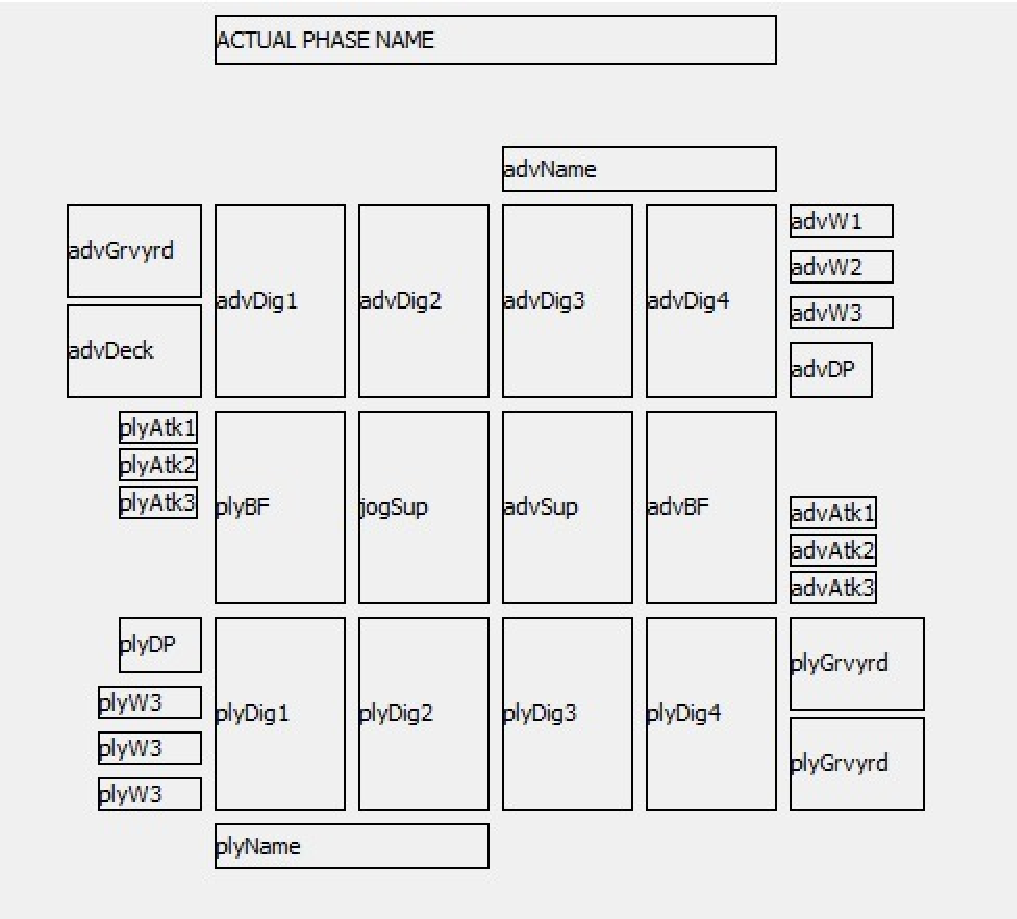
\includegraphics[scale=1]{Prototipo-GUI.pdf}
	\end{figure}
\end{document}